\section{Methods and theory}
The selected model for this project is a recurrent neural network (RNN).
In contrast to feed forward neural networks, an RNN introduces a loop in the network by passing the output (or hidden information) as input for the next step of the network.
This allows the network to maintain a memory of previous outputs of the network, which makes the network suitable for sequence-based domains, such as time-series data and natural language processing.

Figure \ref{fig:unrolled} depicts how the state of an RNN is fed to the next step.
At each step $i$, an input vector $x_i$ is fed into the network, as well as information from the previous state.
For $i=0$, this previous information tends to be initialized either randomly or as a default value.
Given the both inputs, the RNN generates an output $h_i$.
The structure from Figure \ref{fig:unrolled} hints that the prediction of output $h_3$ is based on its direct input $x_3$, but also all its preceding inputs $x_0$, $x_1$ and $x_2$.

\begin{figure}[t]
	\label{fig:unrolled}
	\centering
	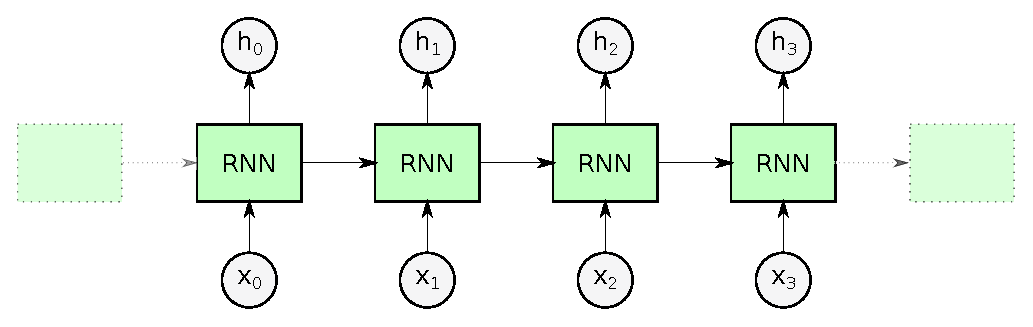
\includegraphics[width=0.6\textwidth]{figures/unrolled.eps} 
	\caption{A generic representation of an RNN. Input $x_i$ and information from the previous step results in output $h_i$.}
\end{figure}

\subsection{Design}
Our proposed RNN accepts an encoding of a character and outputs a probability vector, where each element in the output vector represents the probability of a certain character following the input vector.

Figure \ref{fig:rnn} shows the design of the RNN. The network accepts two inputs: the input, and a hidden state of the previous time step. 
The hidden state is initialized as a vector of zeros for the first step.
Both the input and hidden vectors are one-dimensional. 
The input vector is a one-hot encoding of a single character. 
Therefore, the size of the input vector is defined by the size of the alphabet (i.e. the list of all possible characters).
The size of the hidden vector is one of the hyper-parameters of the network.
The concatenation of the input and hidden vectors is fed to two linear transformation layers (input-to-output {\tt i2o} and input-to-hidden {\tt i2h}). 
The output of {\tt i2h} is the hidden state for the next step of the network.

Both outputs are concatenated and fed in yet another linear transformation layer (output-to-output {\tt o2o}).
The output size is equal to the alphabet size (i.e. the number of unique encountered characters in the training set), such that the output layer can be used as a classifier for the predicted character (i.e. each index in the output layer is the probability for a certain character in the alphabet).
A dropout layer sets values of the output vector to zero with a probability of $p$ (again, a hyper parameter).
The dropout layer serves two functions: (1) prevent overfitting in the training phase and (2) make the network non-deterministic when sampling.
A last softmax layer ensures that the output layer represents a probability density, summing to 1.

\begin{figure}[t]
	\label{fig:rnn}
	\centering
	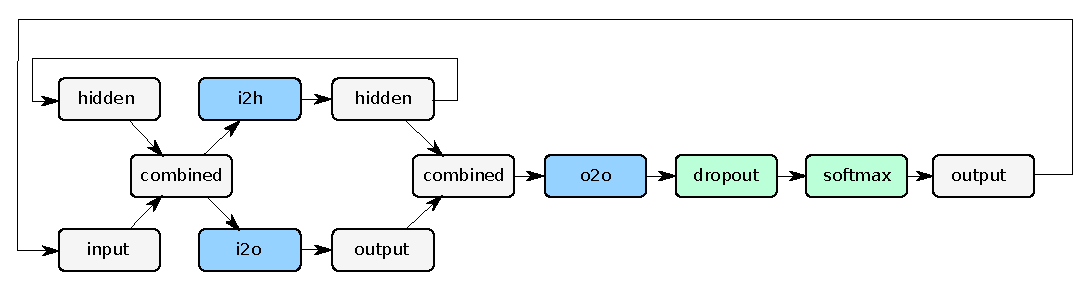
\includegraphics[width=0.75\textwidth]{figures/rnn.eps} 
	\caption{The design of the neural network. The grey boxes are input- and output vectors, the blue boxes represent linear transformation layers and the green boxes are vector transformations applied to the output of the network.}
\end{figure}